% ============================================================
% Section 4: Results
% Author: Them (MS)
% Data source: results/summary.csv (pilot, N=30 issues)
% Script: src/build_summary.py --mode pilot
% ============================================================

\section{Results}
\label{sec:results}

This section reports the quantitative outcomes of the pilot experiment
($N = 30$ GitHub issues, drawn from \textit{pandas}, \textit{scikit-learn},
and \textit{VS Code}).
All metrics were computed by \texttt{src/build\_summary.py} from
\texttt{data/pilot\_ground\_truth.csv} and
\texttt{results/pilot\_llm\_output.csv}.
No LLM responses were excluded ($N_{\text{invalid}} = 0$, invalid rate = 0\%).

% ----------------------------------------------------------------
\subsection{RQ1: Does GPT-4o mini reach $\kappa \geq 0.70$?}
% ----------------------------------------------------------------

Table~\ref{tab:rq1} reports the pooled LLM-vs-Developer Cohen's Kappa
across all three components (OB, EB, S2R combined; $n = 90$ label pairs).
The 95\% confidence interval was obtained via cluster bootstrap
($B = 5\,000$ resamples) resampling at the issue level to account for
the within-issue correlation of OB, EB, and S2R labels.

\begin{table}[h]
\centering
\caption{RQ1 — LLM-vs-Developer Overall Kappa (pilot, $N=30$ issues)}
\label{tab:rq1}
\begin{tabular}{lcccc}
\hline
\textbf{Metric} & \textbf{$\kappa$} & \textbf{95\% CI} & \textbf{Threshold} & \textbf{Decision} \\
\hline
Overall Kappa (pooled) & 0.582 & [0.387, 0.740] & 0.70 & Fail to reject $H_0$ \\
Raw agreement          & 0.844 & —              & —    & Descriptive \\
\hline
\end{tabular}
\end{table}

The point estimate $\kappa = 0.582$ falls below the registered threshold
of 0.70.
The 95\% CI $[0.387, 0.740]$ includes 0.70, indicating that the pilot
sample ($N = 30$) does not provide sufficient statistical power to
conclusively accept or reject $H_1: \kappa \geq 0.70$.

% ----------------------------------------------------------------
\subsection{RQ2: Which component has the highest and lowest agreement?}
% ----------------------------------------------------------------

Table~\ref{tab:rq2} reports per-component LLM-vs-Developer Kappa.
Each component was computed independently on $n = 30$ label pairs.

\begin{table}[h]
\centering
\caption{RQ2 — LLM-vs-Developer Kappa by component (pilot, $N=30$)}
\label{tab:rq2}
\begin{tabular}{lcccc}
\hline
\textbf{Component} & \textbf{$\kappa$} & \textbf{95\% CI} & \textbf{Interpretation} & \textbf{Decision} \\
\hline
OB  & UNDEFINED & [nan, nan]     & —            & See note below \\
EB  & 0.653     & [0.371, 0.902] & Substantial  & PASS ($\geq 0.60$) \\
S2R & 0.400     & [0.148, 0.672] & Fair         & FAIL ($< 0.60$)    \\
\hline
\end{tabular}
\end{table}

\textbf{Note on OB Kappa.}
The developer consensus assigned \textit{Sufficient} to all 30 OB slots
(label distribution: \texttt{Sufficient}: 30/30).
When both raters use only one label, the Cohen's Kappa formula produces
$0/0$ (undefined), not 1.000.
The LLM likewise assigned \textit{Sufficient} to all 30 OB slots,
yielding 100\% raw agreement on OB; however, Kappa is undefined and
is not reported as a numeric value.

Among the two computable components:
\begin{itemize}
  \item \textbf{EB} achieved the highest agreement ($\kappa = 0.653$,
        substantial per Landis \& Koch~\cite{landis1977}).
  \item \textbf{S2R} achieved the lowest agreement ($\kappa = 0.400$,
        fair), with a wide CI $[0.148, 0.672]$ indicating high
        uncertainty at $N = 30$.
\end{itemize}

Figure~\ref{fig:kappa_component} visualizes the per-component Kappa
values with 95\% confidence intervals.

\begin{figure}[h]
\centering
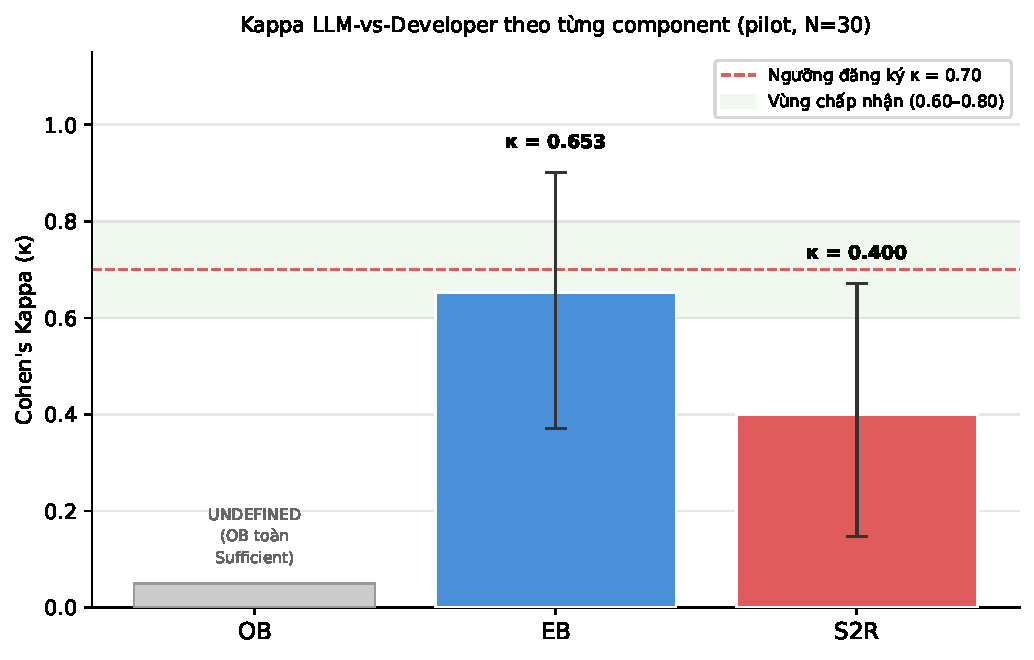
\includegraphics[width=0.75\linewidth]{figures/fig_kappa_by_component}
\caption{LLM-vs-Developer Kappa by component (pilot, $N=30$).
         Dashed line marks the registered threshold $\kappa = 0.70$.
         Error bars show 95\% cluster bootstrap CI.
         OB Kappa is undefined (all labels \textit{Sufficient}).}
\label{fig:kappa_component}
\end{figure}

% ----------------------------------------------------------------
\subsection{Quality Control: Human--Human Inter-Annotator Agreement}
% ----------------------------------------------------------------

Table~\ref{tab:iaa} reports the Human--Human Cohen's Kappa on the
double-labeled subset ($n = 10$ issues, 30\% of pilot sample).

\begin{table}[h]
\centering
\caption{Human--Human Kappa on double-labeled subset ($n=10$)}
\label{tab:iaa}
\begin{tabular}{lcc}
\hline
\textbf{Component} & \textbf{$\kappa$} & \textbf{Note} \\
\hline
OB  & UNDEFINED & All consensus labels are \textit{Sufficient} \\
EB  & UNDEFINED & All consensus labels are \textit{Sufficient} \\
S2R & 1.000     & FLAG --- possible contamination (see Section~\ref{sec:threats}) \\
\hline
\end{tabular}
\end{table}

Human--Human Kappa for OB and EB is undefined for the same reason as
LLM-vs-Developer OB: the pilot sample contains no disagreement on these
components, making Kappa uncomputable.
Human--Human Kappa for S2R equals 1.000, which is flagged for
investigation; a possible explanation is label contamination between
annotators (discussed in Section~\ref{sec:threats}).

% ----------------------------------------------------------------
\subsection{Label Distribution}
% ----------------------------------------------------------------

Table~\ref{tab:dist} shows the label distribution assigned by developer
consensus and the LLM across all three components ($3 \times 30 = 90$
slots).

\begin{table}[h]
\centering
\caption{Label distribution: developer consensus vs.\ LLM (pilot)}
\label{tab:dist}
\begin{tabular}{lcccc}
\hline
\textbf{Label} & \textbf{Consensus} & \textbf{\%} & \textbf{LLM} & \textbf{\%} \\
\hline
Sufficient & 64 & 71.1\% & 74 & 82.2\% \\
Missing    & 23 & 25.6\% & 15 & 16.7\% \\
Ambiguous  &  3 &  3.3\% &  1 &  1.1\% \\
Incorrect  &  0 &  0.0\% &  0 &  0.0\% \\
\hline
\textbf{Total} & \textbf{90} & & \textbf{90} & \\
\hline
\end{tabular}
\end{table}

The distribution is heavily skewed toward \textit{Sufficient}
(71.1\% of consensus labels), resulting in a high chance-agreement
probability ($p_e \approx 0.59$).
This label imbalance explains why the raw agreement of 84.4\% translates
to a substantially lower Kappa of 0.582 --- a known phenomenon referred to
as the \textit{Kappa paradox}~\cite{feinstein1990}.
The LLM assigns \textit{Sufficient} even more frequently than developers
(82.2\% vs.\ 71.1\%), suggesting a systematic bias toward positive
labeling on this pilot sample.
